\documentclass[../main.tex]{subfiles}

%\graphicspath{{\subfix{../images/}}}

\begin{document}

\subsection{Overview}
\begin{table}[!h]
    \centering
    \begin{tabular}{c | c c c c c c}
        $\mathbb{F}$    & GL($n,\mathbb{F}$)    & SL($n,\mathbb{F}$) & U($n$) & SU($n$) & O($n$)     & SO($n$)     \\ \hline\hline
        $\mathbb{R}$    & $n^2$                 & $n^2-1$            & -      & -       & $n(n-1)/2$ & $n(n-1)/2$  \\
        $\mathbb{C}$    & $2n^2$                & $2(n^2-1)$         & $n^2$  & $n^2-1$ & $n(n-1)$   & $n(n-1)$    \\
    \end{tabular}
    \caption{Dimensions of common Lie groups (number of independent real parameters)}
    \label{tab:my_label}
\end{table}
Observation: $\text{dim}(\text{SO}(n,\mathbb{F}))=\text{dim}(\text{O}(n,\mathbb{F}))$  - sign that SO($n$) is not connected

\begin{align}
e^X&=\sum_{n=0}\frac{1}{n!}X^n\\
\text{det}\;e^X&=e^{\text{tr} X} \\
\left(e^X\right)^{-1}&=e^{-X}\\
e^Xe^Y&=e^{X+Y+\frac{1}{2}[X,Y]+\frac{1}{12}[X,[X,Y]]-\frac{1}{12}[Y,[X,Y]]+...}
\end{align}

\subsection{SO(N)}
Defining representation
\begin{align}
O^TO&=1_{N\times N}\\
O&=e^X
\end{align}

\subsection{SO(2)}
Group of rotations in two dimensions - therefore rotations are naturally given by a $2\times2$ matrix $R$ with parameter $\alpha$ (and the generator $X$)
\begin{align}
R=\left(\begin{matrix}
\cos\alpha  & -\sin\alpha\\
\sin\alpha & \cos\alpha
\end{matrix}\right)
\qquad
-iX=\left.\frac{\partial R}{\partial\alpha}\right|_{\alpha=0}=\left(\begin{matrix}
0 & -1\\
1 & 0
\end{matrix}\right)
\end{align}
acting on vectors $(x,y)$. This is therefore also a 2-dimensional (real) representation of SO(2) - it is even an irrep.
In a complex space the vector can be written as $z=x+iy$ and the rotation is represented by $e^{i\alpha}$ - which serves as a one dimensional complex representation.

There are actually infinitely many (non-equivalent) 1-dimensional standard irreps
\begin{align}
    D^{k}(\alpha)=e^{-ik\alpha},\,k=0,\pm1,\pm2,...
\end{align}

\subsection{SO(3) - What we know from quantum mechanics}
The angular momentum algebra is given by $[J_i,J_j]=i\hbar\varepsilon_{ijk}J_k$. We know that
\begin{align}
J^2|jm\rangle&=j(j+1)|jm\rangle\qquad j\in\left\{0,\frac{1}{2},1,\frac{3}{2},...\right\},\quad m=-j,...,j\\
J_z|jm\rangle&=m|jm\rangle
\end{align}
meaning that $J^2$ and $J_3$ can be diagonalized at the same time. For each $j$ there is a $2j+1$ dimensional 
irrep on the Hilbert space. The subspace spanned by the states $\{|jm\rangle\}_{m\in\{-j,...,j\}}$ 
is called $\mathfrak{h}_j$. The states of 
two added angular momenta $j_1$ and $j_2$ are in the space $\mathfrak{h}_{j_1j_2}=\mathfrak{h}_{j_1}\otimes\mathfrak{h}_{j_2}$ spanned by the tensor product of the eigenstates of $(J_{j_1}^2,J_{j_1,3})$ and $(J_{j_2}^2,J_{j_2,3})$
\begin{align}
|j_1m_1j_2m_2\rangle=|j_1,m_1\rangle\otimes|j_2,m_2\rangle
\end{align}
The operators $J^2$, $J_3$, $J_{j_1}^2$ and $J_{j_2}^2$ commute which means they share one set of eigenfunctions $|j_1,j_2,j,m\rangle$ which also spans $\mathfrak{h}_{j_1,j_2}$. Both basis set are connected by the Clebsch-Gordon coefficients
\begin{align}
|j_1,j_2,j,m\rangle=\sum_{m_1,m_2}\langle j_1,m_1,j_2,m_2|j_1,j_2,j,m\rangle|j_1m_1,j_2,m_2\rangle
\end{align}

The dimension of the Product space is given by
\begin{align}
\text{dim}(\mathfrak{h}_{j_1} \otimes \mathfrak{h}_{j_2})&=(2j_1+1)(2j_2+1).
\end{align}
The tensor product representations decomposes as ({\sc Clebsch-Gordan} decomposition)
\begin{align}
    \mathfrak{h}_{j_1} \otimes \mathfrak{h}_{j_1} &\cong \bigoplus_{j=|j_1-j_2|}^{j_1+j_2} \mathfrak{h}_{j}\\
    &=\mathfrak{h}_{j_1+j_2}\oplus \mathfrak{h}_{j_1+j_2-1}\oplus ... \oplus \mathfrak{h}_{j_1-j_2+1}\oplus \mathfrak{h}_{|j_1-j_2|}
\end{align}
Examples
\begin{align}
j_1=\frac{1}{2}, j_2=\frac{1}{2}&\quad\rightarrow\quad 2\otimes2=1\oplus3\\
j_1=1, j_2=1&\quad\rightarrow\quad 3\otimes3=1\oplus3\oplus5
\end{align}

\subsection{SO(3)}

Group of rotations in three dimensions
\begin{align}
v^2
&=\vec{v}^T\vec{v}\\
&=(R\vec{v})^T(R\vec{v})\\
&=\vec{v}^TR^TR\vec{v}\\
&\qquad \rightarrow R^TR=I
\end{align}
therefore rotations around the 3 coordinate axis are naturally given by three  $3\times3$ matrices $R_i$ (with the generators $X_i$)
\begin{align}
R_3=\left(\begin{matrix}
\cos\alpha  & -\sin\alpha & 0\\
\sin\alpha & \cos\alpha & 0\\
0 & 0 & 1 
\end{matrix}\right)
\qquad
-iX_3=\left.\frac{\partial R}{\partial\alpha}\right|_{\alpha=0}=\left(\begin{matrix}
0 & -1 & 0\\
1 & 0  & 0\\
0 & 0  & 0
\end{matrix}\right)\\
R_2=\left(\begin{matrix}
\cos\alpha  & 0 & \sin\alpha\\
0 & 1 & 0\\
-\sin\alpha & 0 & \cos\alpha\\
\end{matrix}\right)
\qquad
-iX_2=\left.\frac{\partial R}{\partial\alpha}\right|_{\alpha=0}=\left(\begin{matrix}
0 & 0  & 1\\
0 & 0  & 0\\
-1 & 0  & 0
\end{matrix}\right)\\
R_1=\left(\begin{matrix}
1 & 0 & 0 \\
0 & \cos\alpha & -\sin\alpha\\
0 & \sin\alpha &  \cos\alpha\\
\end{matrix}\right)
\qquad
-iX_1=\left.\frac{\partial R}{\partial\alpha}\right|_{\alpha=0}=\left(\begin{matrix}
0 & 0  & 0\\
0 & 0  & -1\\
0 & 1  & 0
\end{matrix}\right)
\end{align}  
which also a 3-dimensional representation of SO(3). The generators obey the commutation relation 
\begin{align}
[X_i,X_i]=i\varepsilon_{ijk}X_k
\end{align}

\subsection{SU(2)}
Unitary transformation like a complex rotation - so the condition is
\begin{align*}
U^\dagger U=I\qquad \text{or}\qquad U^\dagger=U^{-1}
\end{align*}
Construction of a generic SU(2) matrix
\begin{align*}
U&=\left(
\begin{matrix}
a & c\\
c & d
\end{matrix}
\right)\qquad ad-bc=1\\
\rightarrow U^{-1}&=\frac{1}{ad-bc}\left(
\begin{matrix}
d & -b\\
-c & a
\end{matrix}
\right)=\left(\begin{matrix}
d & -b\\
-c & a
\end{matrix}
\right)\\
\rightarrow U^\dagger&=\left(
\begin{matrix}
\bar{a} & \bar{c}\\
\bar{b} & \bar{d}
\end{matrix}
\right)
\end{align*}
then with $U^\dagger=U^{-1}$ we have with $a,b \in \mathbb{R}$ and $a\bar{a}+b\bar{b}=a_1^2+a_2^2+b_1^2+b_2^2=1$
\begin{align*}
U&=\left(\begin{matrix}
a & b\\
-\bar{b} & \bar{a}
\end{matrix}
\right)
=\left(\begin{matrix}
a_1+ia_2 & b_1+ib_2\\
-b_1+ib_2 & a_1-ia_2
\end{matrix}
\right)\\
&=a_1\left(\begin{matrix}
1 & 0\\
0 & 1
\end{matrix}
\right)+
a_2i\left(\begin{matrix}
1 & 0\\
0 & -1
\end{matrix}
\right)+
b_1i\left(\begin{matrix}
0 & -i\\
i & 0
\end{matrix}
\right)
+
b_2i\left(\begin{matrix}
0 & 1\\
1 & 0
\end{matrix}
\right)\\
&=a_1I+a_2 i\sigma_3+b_1i\sigma_2+b_2i\sigma_1\\
&=\sqrt{1-a_2^2-b_1^2-b_2^2}I+a_2 i\sigma_3+b_1i\sigma_2+b_2i\sigma_1
\end{align*}
Finding the generators
\begin{align*}
\left.\frac{\partial U}{\partial a_2}\right|_{...=0}=\left.\frac{-2a_2}{2\sqrt{1-a_2^2-b_1^2-b_2^2}}I+i\sigma_3\right|_{...=0}=i\sigma_3\\
\left.\frac{\partial U}{\partial b_1}\right|_{...=0}=\left.\frac{-2b_1}{2\sqrt{1-a_2^2-b_1^2-b_2^2}}I+i\sigma_2\right|_{...=0}=i\sigma_2\\
\left.\frac{\partial U}{\partial b_1}\right|_{...=0}=\left.\frac{-2b_2}{2\sqrt{1-a_2^2-b_1^2-b_2^2}}I+i\sigma_1\right|_{...=0}=i\sigma_1
\end{align*}
The actual generators are
\begin{align*}
Y_k=\frac{i}{2}\sigma_k,\qquad\rightarrow\qquad[Y_i,Y_j]=\epsilon_{ijk}Y_k
\end{align*}

\subsection{SU(3)}

\subsection{Lorentz group O(1,3)}
The generators are a generalisation of the 3d rotations
\begin{align}
J^{\mu\nu}
&=i(x^\mu\partial^\nu-x^\nu\partial^\mu)\\
&=i(x^\mu g^{\alpha\nu}\partial_\alpha-x^\nu g^{\alpha\mu}\partial_\alpha)\\
J^{\mu\nu}x^\rho
&=i(x^\mu g^{\alpha\nu}\delta^\rho_\alpha-x^\nu g^{\alpha\mu}\delta^\rho_\alpha)\\
&=i(\delta^\mu_\sigma x^\sigma g^{\alpha\nu}\delta^\rho_\alpha-\delta^\nu_\sigma x^\sigma g^{\alpha\mu}\delta^\rho_\alpha)\\
&=i(\delta^\mu_\sigma g^{\rho\nu}-\delta^\nu_\sigma g^{\rho\mu})x^\sigma\\
&=(J^{\mu\nu})^\rho_{\;\;\sigma}x^\sigma
\end{align}
meaning there is a four dimensional representation of the Lorentz Lie algebra. 
\begin{align}
(J^{\mu\nu})^\rho_{\;\;\sigma}&=i(\delta^\mu_\sigma g^{\rho\nu}-\delta^\nu_\sigma g^{\rho\mu})\\
\end{align}
Finite-dimensional Representations
\begin{itemize}
\item $\mathbb{R}$ 1-dim - trivial representation $J^{\mu\nu}=0$
\item $\mathbb{R}^4$ 4-dim - vector representation $(J^{\mu\nu})^\rho_{\;\;\sigma}=i(\delta^\mu_\sigma g^{\rho\nu}-\delta^\nu_\sigma g^{\rho\mu})$
\item $\mathbb{R}^6$ 6-dim - adjoint representation $(J^a)^b_{\;\;c}=-if^{ab}_{\;\;\;c}$
\item $\mathbb{C}^2$ 2-dim - left handed Weyl spinor rep. $J^{\mu\nu}=S^{\mu\nu}$ with $S^{ij}=\frac{1}{2}\epsilon^{ijk}\sigma^k$ and $S^{0i}=-\frac{i}{2}\sigma^i$
\item $\mathbb{C}^2$ 2-dim - right handed Weyl spinor rep. $J^{\mu\nu}=S^{\mu\nu}$ with $S^{ij}=\frac{1}{2}\epsilon^{ijk}\sigma^k$ and $S^{0i}=\frac{i}{2}\sigma^i$
\item $\mathbb{C}^4$ 4-dim - Dirac spinor rep. $J^{\mu\nu}=S^{\mu\nu}=\frac{i}{4}[\gamma^\mu,\gamma^\nu]$ 
\end{itemize}
The group elements are $\Lambda=\exp\left(-i\omega_{\mu\nu}J^{\mu\nu}/2\right)$.






There are the obvious tensor representations for tensors of first and second order
\begin{align}
    [D(\Lambda)]^\alpha_{\;\beta}=\Lambda^\alpha_{\;\beta}\quad &\rightarrow\quad V^\alpha = [D(\Lambda)]^\alpha_{\;\beta} V^\beta=\Lambda^\alpha_{\;\beta} V^\beta\\
    [D(\Lambda)]_{\alpha\beta}^{\;\;\gamma\delta}=\Lambda_\alpha^{\;\gamma}\Lambda_\beta^{\;\delta}\quad&\rightarrow\quad T_{\alpha\beta} = [D(\Lambda)]_{\alpha\beta}^{\;\;\gamma\delta} T_{\gamma\delta}=\Lambda_\alpha^{\;\gamma}\Lambda_\beta^{\;\delta}T_{\gamma\delta}
\end{align}
which are 4 and 16 dimensional.

Infinitesimal Lorentz transformations can be written as
\begin{align}
    \Lambda^\alpha_{\;\beta}=\delta^\alpha_{\;\beta}+\omega^\alpha_{\;\beta}\qquad(|\omega^\alpha_{\;\beta}|\ll 1).
\end{align}
The first order approximation gives an additional restriction
\begin{align}
    \eta_{\mu\nu} &= \eta_{\alpha\beta}\Lambda^\alpha_{\;\mu}\Lambda^\beta_{\;\nu}=\eta_{\alpha\beta}(\delta^\alpha_{\;\mu}+\omega^\alpha_{\;\mu})(\delta^\beta_{\;\nu}+\omega^\beta_{\;\nu})=\eta_{\mu\nu}+\eta_{\mu\beta}\omega^\beta_{\;\nu}+\eta_{\alpha\nu}\omega^\alpha_{\;\mu}\\
    &\rightarrow \omega_{\mu\nu}=-\omega_{\nu\mu}
\end{align}
which implies six independent components. As the four dimensional representation of the infinitesimal transformation is close to unity it can then be written as
\begin{align}
    D(\Lambda)=D(1+\omega)=1+\frac{1}{2}\omega^{\alpha\beta}\sigma_{\alpha_\beta}
\end{align}
where the six $\omega$ components correspond to the six matrices $\sigma_{01},\sigma_{02},\sigma_{03},\sigma_{12},\sigma_{13},\sigma_{23}$ which are the generators of the group.


Finite dimensional irreps of the Lorentz group are labeled by two parameters $(\mu,\nu)$ with
\begin{align}
    \mu,\nu &\in \left\{0,\frac{1}{2},1,\frac{3}{2},2,...\right\}.
\end{align}
and have dimension $(2\mu+1)(2\nu+1)$
\begin{align*}
    M^2&=\mu(\mu+1)\\
    N^2&=\nu(\nu+1)\\
    j  &\in |\mu-\nu|, ..., (\mu+\nu)
\end{align*}


\begin{center}
 \begin{tabular}{c c c l} 
 \hline
 irrep & dim & $j$ & example \\ [0.5ex] 
 \hline\hline
 $(0,0)$                        & 1 & 0 & Scalar \\  [0.5ex]
 $(\frac{1}{2},0)$              & 2 & $\frac{1}{2}$ & Left-handed Weyl spinor \\  [0.5ex]
 $(0,\frac{1}{2})$              & 2 & $\frac{1}{2}$ & Right-handed Weyl spinor \\  [0.5ex]
 $(\frac{1}{2},\frac{1}{2})$    & 4 & 0,1 & 4-Vector $A^\mu$ \\  [0.5ex]
 $(1,0)$                        & 3 & 1 & Self-dual 2-form \\  [0.5ex]
 $(0,1)$                        & 3 & 1 & Anti-self-dual 2-form \\  [0.5ex]
 $(1,1)$                        & 9 & 0,1,2 & Traceless symmetric $2^\text{nd}$ rank tensor \\ \hline  \\ [0.5ex]
  \hline
 rep & dim & j & example \\ [0.5ex] 
 \hline\hline
 $(\frac{1}{2},0)\oplus(0,\frac{1}{2})$& - & - & Dirac bispinor $\psi^\alpha\quad \alpha\in\{1,2,3,4\}$ \\  [0.5ex]
 $(\frac{1}{2},\frac{1}{2})\otimes\left[(\frac{1}{2},0)\oplus(0,\frac{1}{2})\right]=(1,\frac{1}{2})\otimes(\frac{1}{2},1)$& - & - & Rarita-Schwinger field $\psi^\alpha\quad \alpha\in\{1,2,3,4\}$ \\  [0.5ex]
  $(1,0)\oplus(0,1)$& - & - & Parity invariant field of 2-forms\\  [0.5ex]
  $(\frac{3}{2},0)\oplus(0,\frac{3}{2})$& - & - & Gravitino \\ \hline \\ [0.5ex]
\end{tabular}
\end{center}

% LORENTZ GROUP (DOUBLE COVER) REPRESENTATIONS
% Inspired by https://arxiv.org/abs/1705.02227 (V.V. Varlamov)
% https://en.wikiversity.org/wiki/Representation_theory_of_the_Lorentz_group#Common_representations
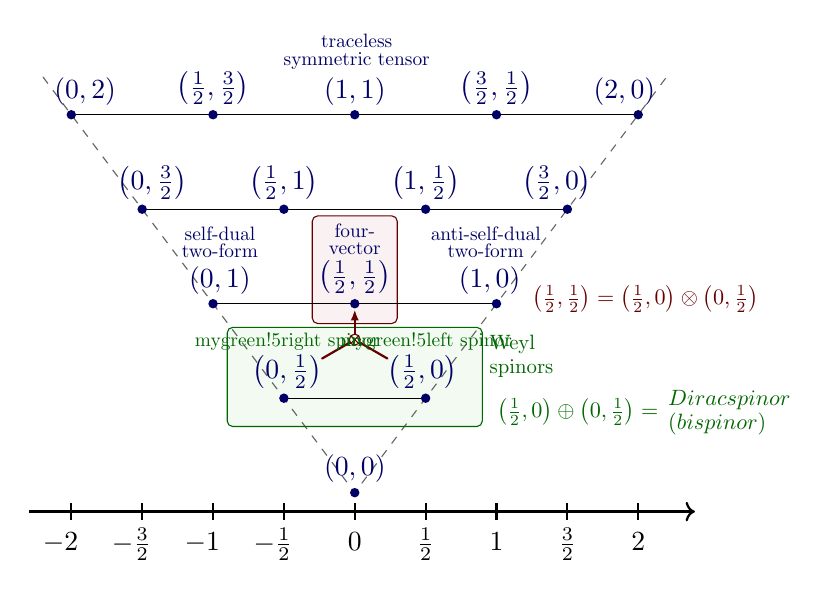
\begin{tikzpicture}[x=1.8cm,y=1.2cm]
\usetikzlibrary{arrows.meta} % to control arrow size
\contourlength{1.2pt}
\newcommand\LP{{\color{mydarkblue}P}} %\Lambda_\mathrm{P}
\newcommand\LT{{\color{mydarkred}T}} %\Lambda_\mathrm{T}
\colorlet{myred}{red!60!black}
\colorlet{myblue}{blue!60!black}
\colorlet{mygreen}{green!60!black}
\colorlet{mydarkblue}{blue!40!black}
\colorlet{mydarkred}{red!40!black}
\colorlet{mydarkgreen}{green!40!black}
\colorlet{mydarkpurple}{blue!50!red!50!black}
\tikzstyle{myarr}=[-{Latex[length=4,width=3]}]


  \def\N{4}      % number of spin states
  \def\r{0.07cm} % radius otimes
  \def\repr#1{   % format simple fraction
    \pgfmathsetmacro{\double}{int(2*#1)}
    \pgfmathsetmacro{\sign}{ifthenelse(#1<0,"-","")}
    \pgfmathparse{int(mod(\double,2))}
    \ifnum0=\pgfmathresult\relax % even
      \pgfmathprintnumber{#1}
    \else % odd
      \sign % sign
      \pgfmathparse{abs(int(\double))}
      \frac{\pgfmathprintnumber{\pgfmathresult}}{2}
    \fi
    \phantom{\sign} % for centered alignment
  }
  
  % AXIS
  \begin{scope}[shift={(0,-0.2)}]
    \draw[->,thick] (-\N/2-0.3,0) -- (\N/2+0.4,0); %node[right=-1] {$S$};
    \foreach \j [evaluate={\x=\j/2; \m=\j/2;}] in {-\N,...,\N}{ % ticks
      \draw[thick] (\x,0.09) --++ (0,-0.18)
        node[below=-1] {\strut$\repr{\m}$}; 
    }
  \end{scope}
  
  % LABELS Dirac spinor
  \draw[dashed,opacity=0.6] (-1.1*\N/2,1.1*\N) -- (0,0) -- (1.1*\N/2,1.1*\N);
  \draw[mydarkgreen,fill=mygreen,fill opacity=0.05,rounded corners=2]
    (-0.9,0.7) rectangle (0.9,1.75)
    node[mydarkgreen,below right,align=left,opacity=1,scale=0.75] {Weyl\\spinors};
  \node[mydarkgreen,scale=0.8,below right] at (0.95,1.2)
    {$\left(\frac{1}{2},0\right)\oplus\left(0,\frac{1}{2}\right)
       = \!\! \begin{array}{l}
           \text{Dirac spinor}\\[-0.5mm]
           \text{(bispinor)}
         \end{array}$};
  %\node[mydarkgreen,scale=0.8,below,align=center] at (1.55,0.68)
  %  {Dirac spinor\\[-3](bispinor)};
  %\node[mydarkgreen,scale=0.8,below,align=center] at (2.58,0.68)
  %  {four-\\[-3]vector};
  %\node[mydarkgreen,scale=0.8,below right] at (1.5,2.2)
  %  {$(1,0)\oplus(0,1) = \text{adjoint}$}; % parity-invariant 2-form field
  
  % LABELS four-vector
  \draw[mydarkred,fill=myred,fill opacity=0.05,rounded corners=2]
    (-0.3,1.79) rectangle (0.3,2.93);
  \node[mydarkred,scale=0.8,right] at (1.2,2.05)
    {$\left(\frac{1}{2},\frac{1}{2}\right) = %\cong
      \left(\frac{1}{2},0\right)\otimes\left(0,\frac{1}{2}\right)$};
  
  % DOTS
  \foreach \j [evaluate={\y=\j;}] in {0,...,\N}{
    \draw (-\j/2,\y) --++ (\j,0);
    \foreach \i [evaluate={
      \m=\i-\j/2;
      \L=\i/2; % left representation
      \R=\j/2-\i/2; % right representation
      \x=\m; % x position
      \myshift=((\i==0||\i==\j)?-2.5*\x:0);
    }] in {0,...,\j}{
      \fill[mydarkblue] (\x,\y) circle (0.06cm);
      \node[mydarkblue,right=\myshift,above]
        %,fill=white,text opacity=1,fill opacity=0.5,inner sep=0.5,outer sep=3
        (P\j-\i) at (\x,\y) {$\left(\repr{\L},\repr{\R}\right)$};
    }
  }
  
  % ARROWS & OTIMES
  \draw[thick,mydarkred,line cap=round]
    (-0.23,1.42) -- (0,1.62) coordinate (A) -- (0.23,1.42);
  \draw[myarr,thick,mydarkred,line cap=round]
    (A) -- (0,1.94);
  \draw[mydarkred,line width=0.4,fill=mygreen!5] % circle
    (A) circle(\r);
  \draw[mydarkred,line width=0.4] % cross
    (A)++(45:\r) --++ (-135:2*\r)
    (A)++(135:\r) --++ (-45:2*\r);
  
  % LABELS
  \node[mydarkgreen,scale=0.7,above=6]
    at (P1-0) {\strut\contour{mygreen!5}{right spinor}};
  \node[mydarkgreen,scale=0.7,right=2,above=6]
    at (P1-1) {\strut\contour{mygreen!5}{left spinor}};
  \node[mydarkblue,scale=0.7,above=8,align=center]
    at (P2-0) {self-dual\\[-3]two-form};
  \node[mydarkblue,scale=0.7,above=8,align=center]
    at (P2-1) {four-\\[-3]vector};
  \node[mydarkblue,scale=0.7,left=2,above=8,align=center]
    at (P2-2) {anti-self-dual\\[-3]two-form};
  \node[mydarkblue,scale=0.7,right=1,above=8,align=center]
    at (P4-2) {traceless\\[-3]symmetric tensor};
  
\end{tikzpicture}

\end{document}